%% =====================================================================
%% Replicating a paper --- course template (SSRN format)
%% ML & FinTech, National Yang Ming Chiao Tung University
%% Instructor: Huei-Wen Teng
%%
%% Straight replication of Feng et al. (2019), no extension.
%% Every instruction left in \inst{...} is italic; delete it once acted on.
%% =====================================================================

\documentclass[12pt]{article}

\usepackage{adjustbox,array,amssymb,amsmath,amsfonts,eurosym,geometry,graphicx,
            caption,color,setspace,sectsty,comment,footmisc,natbib,pdflscape,
            subfigure,longtable,lscape,float,multirow,booktabs,makecell,
            hyperref,ulem,appendix}

\normalem
\onehalfspacing

\newtheorem{theorem}{Theorem}
\newtheorem{corollary}[theorem]{Corollary}
\newtheorem{proposition}{Proposition}
\newenvironment{proof}[1][Proof]{\noindent\textbf{#1.} }{\ \rule{0.5em}{0.5em}}

\newtheorem{hyp}{Hypothesis}
\newtheorem{subhyp}{Hypothesis}[hyp]
\renewcommand{\thesubhyp}{\thehyp\alph{subhyp}}

\newcolumntype{L}[1]{>{\raggedright\let\newline\\arraybackslash\hspace{0pt}}m{#1}}
\newcolumntype{C}[1]{>{\centering\let\newline\\arraybackslash\hspace{0pt}}m{#1}}
\newcolumntype{R}[1]{>{\raggedleft\let\newline\\arraybackslash\hspace{0pt}}m{#1}}

\geometry{left=1.0in,right=1.0in,top=1.0in,bottom=1.0in}

%% ---------------------------------------------------------------------
%% Instructions are italic. Delete the \inst{...} once you have done it.
%% ---------------------------------------------------------------------
\newcommand{\inst}[1]{\textit{#1}}

\begin{document}

\begin{titlepage}

\title{Replicating the paper:
       Temporal Relational Ranking for Stock Prediction \citep{feng2019temporal}}

\author{Yue Zhen Huang\thanks{Department of Information Management and Finance,
        National Yang Ming Chiao Tung University.}}

\date{\today}
\maketitle

\begin{abstract}
\noindent
Stock returns are usually modeled from each stock's own history, although firms linked through
an industry, a supply chain, or common owners tend to move together.
\citet{feng2019temporal} close this gap with Relational Stock Ranking (RSR), which passes
information between related stocks through a Temporal Graph Convolution and ranks stocks by
next-day return, and they report gains over relation-blind baselines. This replication retrains
the paper's relation-blind Rank\_LSTM and its industry-relation RSR on the authors' released
NASDAQ data and code, under a matched 50-epoch schedule, and repeats the comparison in a second
run. Mean-squared error is indistinguishable between the two models, and the baseline has the
higher top-pick reciprocal rank, as in the paper's own NASDAQ results; the investment return
favors RSR in both of our runs, opposite to the paper, but it is too noisy to settle the
direction. We are interested in this paper because we are building a multi-agent trading system
whose agents each analyze one stock in isolation, and we want to know whether a relation graph
adds a signal before wiring one in.

\vspace{0in}
\noindent\textbf{Keywords:} Stock Prediction, Learning to Rank, Graph-based Learning

\vspace{0in}
\noindent\textbf{JEL Codes:} G17, C45, C53\footnote{\citet{feng2019temporal} do not report JEL
codes, so we chose these ourselves from the JEL classification system: G17 (Financial
Forecasting and Simulation), C45 (Neural Networks and Related Topics), and C53 (Forecasting and
Prediction Methods; Simulation Methods).}

\bigskip
\end{abstract}

\setcounter{page}{0}
\thispagestyle{empty}
\end{titlepage}
\pagebreak

\newpage
\clearpage


\section{Motivation}
\label{sec:motivation}

A stock's future return is usually modeled from its own history, which discards information that
is easy to observe: companies in the same industry, supply chain, or fund tend to move together,
because a shock to one is often a shock to the group. Empirical finance shows that information
travels along such links and reaches prices with a delay. Customer and supplier industries
cross-predict each other's returns \citep{menzly2010market}, news about economically linked firms
is priced slowly \citep{cohen2008economic}, and money managers' commodity-futures positions
predict producers' stock returns the following week \citep{ho2023smart}. Links also shape real
outcomes: upstream tariff cuts raise downstream investment \citep{martin2024downstream}, and
shared institutional owners change supply-chain relationships \citep{freeman2025overlapping}. If
links carry information, a model that treats each stock as an independent series ignores part of
the signal, and the question is whether encoding the links improves prediction.

\citet{feng2019temporal} answer with Relational Stock Ranking (RSR). A graph of relations between
stocks, either shared sector--industry membership or Wikidata facts on ownership, supply, and
competition, enters a Temporal Graph Convolution layer on top of an LSTM encoding of each stock's
price history. The model is trained to rank stocks by next-day return rather than to regress it,
since a trading strategy cares about relative order more than exact values. The paper compares
RSR with a relation-blind LSTM ranker (Rank\_LSTM), a graph-regularized regressor (GBR), and a
plain graph convolution (GCN) on NASDAQ and NYSE. Its claims are conditional. With industry
relations RSR beats Rank\_LSTM on NYSE but not on NASDAQ, which the authors attribute to NASDAQ
being more volatile and dominated by short-term factors; with Wikidata relations it reaches an
investment return ratio of 1.19 against 0.68 for Rank\_LSTM on NASDAQ (their Tables 6 and 7).

Other machine-learning work builds on the same idea. \citet{cui2023temporal} extend pairwise
relations to group-wise hypergraphs of industry belonging and fund holding with hierarchical
attention, and \citet{jafari2022gcnet} apply a graph convolutional network to a stock-relation
graph. \citet{evgeniou2023uncovering} use machine learning to show that firm-level return
predictability is sparse and heterogeneous, so which firms carry signal for which others is an
empirical matter, and \citet{feng2024deep} use deep learning to build latent factors from firm
characteristics.
We set out to reproduce the paper's NASDAQ, industry-relation comparison between Rank\_LSTM and
RSR, using the authors' released data and code. We could obtain the same NASDAQ data and the
same relation graph. We could not obtain the authors' pretrained sequential embedding that RSR
starts from, so we exported it from our own baseline run; we did not tune hyperparameters as the
authors did; and we did not run NYSE, Wikidata relations, or the GBR and GCN comparators. A
reader learns three things the paper alone does not show: how the two models compare under one
fixed, matched schedule; how large run-to-run variation is for each metric; and which defects in
the released data a reproducer must find first (Section~\ref{sec:data}).

Our interest comes from outside this course. We are building a multi-agent system for trading
decisions in which each agent analyzes one stock along one dimension (technical, news, risk).
No agent sees the relationship between stocks, which is the assumption RSR argues against.
Replicating RSR is a first check of whether that signal is real before any such agent is added.
This project does not attempt that integration or extend RSR.

\subsection{Research question}

\begin{itemize}
  \item \textbf{RQ1 (replication).} On the NASDAQ universe with industry relations, does RSR
  improve next-day return ranking relative to Rank\_LSTM, which treats stocks independently?
\end{itemize}


\section{Data}
\label{sec:data}

We use the NASDAQ portion of the dataset released with \citet{feng2019temporal}: daily features
for 1{,}026 tickers over 1{,}246 trading days (January 2013 to December 2017) and a static
industry relation tensor. The repository describes its raw pull as thirty years of data on more
than 8{,}000 stocks. The modeling sample is about five years, and only 1{,}026 stocks pass the
paper's liquidity and history filters. Our data is the authors' own, so it does not differ from
the original paper's data.

\subsection{Dependent and independent variables}

Table~\ref{tab:vars} lists the variables. The response is the next-day return ratio. The
predictors are the closing price, normalized by the stock's maximum over the sample, and its
5-, 10-, 20-, and 30-day moving averages. The model reads the last four days of these five
features. The relation graph is a fixed input shared by all dates.

\begin{table}[h]
\centering
\caption{Variables.}
\label{tab:vars}
\begin{tabular}{lp{8.6cm}l}
\toprule
Acronym & Description & Type \\
\midrule
RET & Response: next-day return ratio, $(p_{t+1}-p_t)/p_t$, which the models predict and rank
across stocks & continuous \\
CLOSE & Closing price divided by the stock's maximum over 2013--2017 & continuous \\
MA5, MA10, MA20, MA30 & 5-, 10-, 20-, 30-day moving averages of the normalized close
& continuous \\
IND & Relation graph: $1{,}026\times1{,}026\times97$ one-hot tensor of shared industry
membership & binary \\
\bottomrule
\end{tabular}
\end{table}

\subsection{Data exploration, cleaning and preprocessing}

Exploratory analysis (notebook \texttt{eda.ipynb}) found three issues.

\begin{enumerate}
  \item \textbf{Missing values are not \texttt{NaN}.} The pipeline (\texttt{preprocess/eod.py})
  pads missing trading days with $-1234$. Left in, the sentinel drives raw skewness to about
  $-23$ for every feature column. Stripped, it falls to between $-0.3$ and $-0.4$, a
  mild skew in a bounded ratio. The sentinel marks only 0.17\% of ticker-days (2{,}202 of
  1{,}278{,}396 rows), yet it dominates any unfiltered statistic. We treat it as missing
  wherever it appears; because so few rows are affected, we add no missing indicator.
  \item \textbf{The graph includes non-company tickers.} 156 of 1{,}026 tickers (15.2\%) have
  industry ``n/a''. They are ETFs and index funds (e.g.\ \texttt{QQQ}, \texttt{SHV}) whose
  return is a basket average with no industry relation, and 17 of them are isolated in the
  graph. We keep them, as the paper does, because dropping them changes the graph; the effect is
  untested.
  \item \textbf{The graph differs from the paper's description.} The tensor has 97 industry
  channels and 5.2\% related stock pairs. The paper's Table 4 reports 112 relation types and
  5.00\%. We could not account for the gap in types.
\end{enumerate}

Next-day return ratios range from $-0.48$ to $0.98$, and only 0.05\% exceed 0.2 in absolute
value. The authors' ticker filter already caps daily returns near 0.98, we did not trace
individual extremes to the source, and we kept them, as the paper does. The features are already
scaled by each stock's maximum price, so we did not rescale.


\section{Methodology}
\label{sec:methods}

\subsection{Benchmark model}

We use the paper's own benchmark, Rank\_LSTM. A single-layer LSTM reads each stock's last
$S=4$ days of features and predicts next-day return from the final hidden state, with no
information exchanged between stocks. This is the ``stocks are independent'' model that RSR is
designed to beat. The relational model is RSR with implicit relation modeling (RSR\_I in the
paper). It takes the baseline's learned sequence embedding and re-weights it over each stock's
neighbors in the industry graph with a learned, softmax-normalized attention, then combines the
propagated and original embeddings for the prediction. The graph is a training-time constant.
Both models use the loss
\[
\mathcal{L} = \lVert \hat{\mathbf r}_{t+1}-\mathbf r_{t+1}\rVert^2
 + \alpha\sum_{i,j}\max\bigl(0,-(\hat r^{\,i}_{t+1}-\hat r^{\,j}_{t+1})(r^{\,i}_{t+1}-r^{\,j}_{t+1})\bigr),
\]
a regression term plus a pairwise penalty for stock pairs whose predicted order contradicts the
realized order.

\subsection{Experimental Design}

Figure~\ref{fig:flow} shows the procedure from raw data to the reported numbers.

\begin{figure}[htbp]
\centering
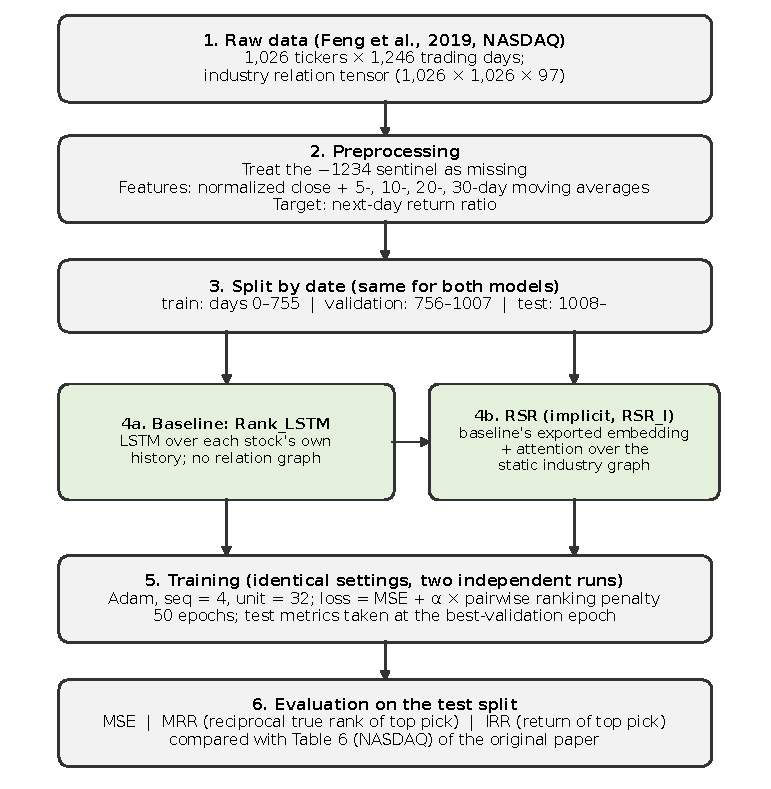
\includegraphics[width=0.78\textwidth]{figures/flowchart.pdf}
\caption{Experimental design, from raw data to reported test-set metrics.}
\label{fig:flow}
\end{figure}

Both models share the date split of the paper (756 training, 252 validation, and the remaining
test days), optimizer (Adam, learning rate 0.001), $\text{seq}=4$, $\text{unit}=32$, and
$\alpha=1$, and both train for 50 epochs. We report test metrics at the epoch with the best
validation loss. The paper tuned hyperparameters by grid search on the investment return and
averaged five test runs; the repository's example command for Wikidata relations uses $\text{seq}=16$ and
$\text{unit}=64$. Our contribution is not a new method but a test the paper does not report: a
matched-schedule comparison, repeated in a second independent run (a new baseline run, hence a
new embedding, and RSR with a different random seed), so that run-to-run variation is visible.

\subsection{Performance measures}

We use the paper's three measures. \emph{MSE} is the mean squared error of predicted return
across stocks and test days. \emph{MRR} is the mean over test days of the reciprocal of the
true-return rank of the model's top-ranked stock (in the code, \texttt{mrrt}). \emph{IRR} is the
cumulative investment return ratio, the sum of the realized next-day returns of the top-ranked
stock over the test days. The code reports \texttt{btl}, which equals one plus this sum, so we
report $\text{IRR}=\texttt{btl}-1$ to match the paper's scale. The paper notes that IRR swings
widely because swapping the top two stocks on one high-return day changes it greatly; we
therefore treat IRR as the noisiest of the three.


\section{Results}
\label{sec:results}

Table~\ref{tab:main} puts the paper's NASDAQ industry-relation results beside ours. The paper
averages five test runs; we have two independent runs.

\begin{table}[h]
\centering
\caption{NASDAQ, industry relations: original paper (Table 6; mean $\pm$ s.d.\ over five test
runs) and this replication (50 epochs, test metrics at best validation epoch). MSE in
$10^{-4}$.}
\label{tab:main}
\begin{tabular}{llccc}
\toprule
Source & Model & MSE ($10^{-4}$) & MRR & IRR \\
\midrule
Paper & Rank\_LSTM & $3.79\pm0.01$ & $0.0417\pm0.0075$ & $0.68\pm0.60$ \\
Paper & RSR\_I & $3.80\pm0.01$ & $0.0317\pm0.0051$ & $0.23\pm0.27$ \\
\midrule
Replication, run 1 & Rank\_LSTM & 3.774 & \textbf{0.0488} & 0.018 \\
Replication, run 1 & RSR\_I & 3.774 & 0.0276 & \textbf{0.130} \\
\midrule
Replication, run 2 & Rank\_LSTM & 3.773 & \textbf{0.0322} & $-0.205$ \\
Replication, run 2 & RSR\_I & 3.787 & 0.0301 & \textbf{0.405} \\
\bottomrule
\end{tabular}
\end{table}

\textbf{MSE replicates.} The two models agree to within 0.4\% in both runs, as in the paper
(3.79 against 3.80). A relation graph does not lower prediction error here.

\textbf{MRR replicates in direction.} The baseline has the higher MRR in both runs, as in the
paper, though the size of the gap varies (0.021 in run 1, 0.002 in run 2, against 0.010 in the
paper). The gap in run 2 is well inside the paper's standard deviations.

\textbf{IRR does not replicate, but cannot decide the question.} RSR has the higher IRR in both
runs, the reverse of the paper's ordering (0.23 against 0.68). Yet the baseline's IRR moves from
0.018 to $-0.205$ between our two runs, and RSR's from 0.130 to 0.405, swings as large as the
paper's own standard deviations (0.60 and 0.27). Two runs cannot establish the sign of a
difference this noisy.

So the answer to RQ1 on NASDAQ with industry relations is no for MSE and MRR and unresolved for
IRR. This agrees with the paper's own statement that industry relations help less on NASDAQ.
Four things may account for the IRR difference, none of which we can separate with two runs:
we did not grid-search hyperparameters on IRR as the authors did; we used two runs, not five;
and the embedding was exported from our own baseline run, not the authors' file, so its
training may differ.


\section{Conclusion}
\label{sec:conclusion}

What survives the replication is the paper's NASDAQ industry-relation finding in its weaker
form: a static industry graph leaves mean-squared error unchanged and does not improve the
ranking of the single best stock, both of which the original Table 6 also shows. The released
code and data were enough to reproduce this, once two traps were cleared: the undocumented
$-1234$ missing-value code, and an embedding file that the repository does not ship.

What a reader should believe less is any claim that RSR raises investment return on NASDAQ from
industry relations alone. The sign of our IRR difference is the opposite of the paper's, and
both are small next to run-to-run variation, so neither supports a conclusion. Needed next are
more seeds, a hyperparameter search toward the paper's configuration, and the Wikidata relation,
where the paper's own NASDAQ gain is largest. For the multi-agent system that motivated this
project, the practical reading is that a static industry graph is not a reliable source of an
extra signal on NASDAQ; whether a richer relation is, remains untested here.


\section*{Declaration}

\subsection*{Declaration of Pedagogical Purpose}

This manuscript is prepared as part of the course project for Machine Learning and
FinTech at National Yang Ming Chiao Tung University, instructed by Professor
Huei-Wen Teng. The work is intended solely for pedagogical purposes, including
learning, discussion, and academic training. It does not represent original research
submitted for journal publication, nor should it be considered professional financial
advice.

\subsection*{Declaration of generative AI and AI-assisted technologies in the writing process}

During the preparation of this work, the authors used Claude, developed by Anthropic, in order
to improve the clarity, precision, and overall quality of the writing and to assist with code
and analysis. After using this tool, the authors reviewed and edited the content as needed and
take full responsibility for the content of the article.


\bibliographystyle{chicago}
\bibliography{ref}


\appendix

\section{Reproduction notes}

Training code is the official repository's \texttt{rank\_lstm.py} and
\texttt{relation\_rank\_lstm.py}, with TensorFlow~1 calls run under TensorFlow~2 and the
environment variable \texttt{TF\_USE\_LEGACY\_KERAS=1} set; without it the scripts fail at
\texttt{BasicLSTMCell}. We added a \texttt{--save\_emb} option to the baseline to export the
sequence embedding and an \texttt{--epochs} option to both. Run 1 uses the default seed. In run 2
the baseline script has no seed option, so it differs from run 1 through initialization alone,
and RSR was run with \texttt{--seed 2} on run 2's embedding. Logs are in \texttt{coding/logs/}.


\end{document}
